\documentclass[aspectratio=169,11pt]{beamer}

% Theme and colors
\usetheme{Madrid}
\usecolortheme{whale}
\setbeamertemplate{navigation symbols}{}
\setbeamertemplate{footline}[frame number]

% Packages
\usepackage[utf8]{inputenc}
\usepackage[T1]{fontenc}
\usepackage{graphicx}
\usepackage{booktabs}
\usepackage{amsmath}
\usepackage{hyperref}
\usepackage{tikz}
\usetikzlibrary{shapes,arrows,positioning,calc,fit,backgrounds,decorations.pathmorphing,patterns}
\usepackage{siunitx}
\usepackage{xcolor}
\usepackage{array}
\usepackage{multirow}

% Custom colors
\definecolor{questionbg}{RGB}{255,248,220}
\definecolor{questionborder}{RGB}{255,193,7}
\definecolor{milestonebg}{RGB}{220,235,255}
\definecolor{milestoneborder}{RGB}{0,100,200}
\definecolor{delivbg}{RGB}{220,255,220}
\definecolor{delivborder}{RGB}{40,167,69}

% Title information
\title[EECE5155 -- Weeks 11--16]{Course Roadmap: Weeks 11--16}
\subtitle{From MVP to Final Demo}
\author{Eduardo Baena}
\date{Spring 2026}
\institute{Northeastern University\\Department of Electrical and Computer Engineering\\
\texttt{e.baena@northeastern.edu}}

\begin{document}

% Title slide
\begin{frame}
    \titlepage
    \vspace{-1cm}
    \begin{center}
        \textbf{EECE5155: Wireless Sensor Networks and the Internet of Things}
    \end{center}
\end{frame}

%==============================================================================
\section{Where We Are}
%==============================================================================

\begin{frame}{Where We Are (End of Week 10)}
    \textbf{What you have learned:}

    \vspace{0.2cm}
    \begin{columns}
        \column{0.5\textwidth}
        \textbf{Modules completed:}
        \begin{enumerate}
            \item[\checkmark] \textbf{Mod 1--2:} Data Acquisition + PES
            \item[\checkmark] \textbf{Mod 3:} Embedded Computing (MCU/SBC)
            \item[\checkmark] \textbf{Mod 4:} Comms (Physical $\rightarrow$ Network)
            \item[\checkmark] \textbf{Mod 5:} Network Layer
            \item[\checkmark] \textbf{Mod 6:} Data Streaming (MQTT, CoAP)
            \item[\checkmark] \textbf{Mod 7:} Data Storage (InfluxDB, Parquet)
            \item[\checkmark] \textbf{Mod 8:} Data Analytics
        \end{enumerate}

        \column{0.5\textwidth}
        \textbf{What remains:}
        \begin{itemize}
            \item \textbf{Mod 9:} AI/MLOps for IoT (Week 11)
            \item \textbf{Cloud IoT Seminar:} hands-on MQTT + InfluxDB + Grafana
            \item \textbf{Hardware MVP:} working sensor-to-cloud prototype
            \item \textbf{Final Integration:} full pipeline running
            \item \textbf{Final Report + Demo:} professional delivery
        \end{itemize}
    \end{columns}

    \vspace{0.2cm}
    \begin{alertblock}{The Shift}
        Lectures are over after Week 11. From Week 12 on, all sessions are \textbf{project-focused}: studios, clinics, and reviews. You must execute, not just learn.
    \end{alertblock}
\end{frame}

%==============================================================================
\section{Week 10 -- This Week}
%==============================================================================

\begin{frame}{Week 10: Wrapping Up Data Analytics}
    \begin{center}
    \footnotesize
    \begin{tabular}{lll}
        \toprule
        \textbf{Date} & \textbf{Session} & \textbf{What Happens} \\
        \midrule
        Mon 03/09 & Data Analytics (Lecture) & Module 8 lecture \\
        Tue 03/11 & Data Analytics (cont.) & Module 8 wrap-up \\
        \textbf{Wed 03/12} & \textbf{Workshop Studio} & \textbf{Finish Module 8 + present roadmap Weeks 11--16} \\
        \bottomrule
    \end{tabular}
    \normalsize
    \end{center}

    \vspace{0.3cm}
    \textbf{Today (Wednesday 03/12):}
    \begin{itemize}
        \item Wrap up Data Analytics (Module 8)
        \item Present the course roadmap for Weeks 11--16
        \item Preview: what the final demo and report look like
        \item \textbf{Start thinking about your MVP:} what hardware do you need?
    \end{itemize}

    \vspace{0.2cm}
    \begin{alertblock}{Looking ahead}
        Next week (Week 11): AI/MLOps lectures Mon--Tue.\\[0.1cm]
        \textbf{MVP Hardware Spec due Wed 03/19.} Thu 03/20: Cloud IoT hands-on seminar.
    \end{alertblock}
\end{frame}


%==============================================================================
\section{Week 11: AI/MLOps + MVP Spec + Cloud IoT Seminar}
%==============================================================================

\begin{frame}{Week 11: AI/MLOps + MVP Spec + Cloud IoT Seminar}
    \begin{center}
    \footnotesize
    \begin{tabular}{lll}
        \toprule
        \textbf{Date} & \textbf{Session} & \textbf{What Happens} \\
        \midrule
        Mon 03/16 & AI/MLOps for IoT (Lecture) & Module 9: pipelines, TinyML, drift, OTA \\
        Tue 03/18 & AI/MLOps (cont.) & Module 9 wrap-up \\
        \textbf{Wed 03/19} & \textbf{MVP Hardware Spec due} & \textbf{Submit BOM on Canvas by end of day} \\
        \textbf{Thu 03/20} & \textbf{Cloud IoT Hands-On Seminar} & \textbf{MQTT + InfluxDB + Grafana lab} \\
        \bottomrule
    \end{tabular}
    \normalsize
    \end{center}

    \vspace{0.3cm}
    \textbf{Thursday Seminar: IoT Cloud Pipeline (1h hands-on)}

    \vspace{0.1cm}
    \begin{enumerate}
        \item \textbf{0--20 min: MQTT} --- Mosquitto broker, publish/subscribe with Python, MQTT Explorer
        \item \textbf{20--40 min: Storage} --- InfluxDB setup, MQTT-to-InfluxDB bridge in Python
        \item \textbf{40--60 min: Dashboard} --- Grafana connected to InfluxDB, one live panel + alert
    \end{enumerate}

    \vspace{0.1cm}
    \begin{exampleblock}{Prerequisites (install before Thursday)}
        Mosquitto, Python 3.10+, paho-mqtt, InfluxDB 2.x, Grafana, MQTT Explorer.\\
        Docker alternative: \texttt{\scriptsize docker run -d -p 1883:1883 eclipse-mosquitto:2 \&\& docker run -d -p 8086:8086 influxdb:2 \&\& docker run -d -p 3000:3000 grafana/grafana-oss}
    \end{exampleblock}
\end{frame}

\begin{frame}{MVP Hardware Spec: Due Wednesday March 19}
    \begin{center}
    \fcolorbox{milestoneborder}{milestonebg}{
    \begin{minipage}{0.85\textwidth}
        \vspace{0.2cm}
        \centering
        \large\textbf{Deliverable: MVP Hardware Specification}

        \vspace{0.2cm}
        \normalsize
        Due: \textbf{Wednesday March 19, end of day} (submit on Canvas)

        \vspace{0.2cm}
        Submit a 1-page document listing:
        \begin{enumerate}
            \item What sensor(s) you need (part number, datasheet link)
            \item What MCU/SBC you are using (already have or need to order)
            \item What communication module (WiFi, BLE, LoRa, etc.)
            \item \textbf{Bill of Materials} with prices (budget: \$50 max, excluding Raspberry Pi)
            \item What you already have vs.\ what the instructor needs to order
        \end{enumerate}

        \vspace{0.1cm}
        \textit{I will review over the weekend and order so you have parts by Week 12.}
        \vspace{0.2cm}
    \end{minipage}
    }
    \end{center}

    \vspace{0.1cm}
    \textbf{Template:}
    \begin{center}
    \scriptsize
    \begin{tabular}{p{3cm}p{2cm}p{2cm}p{1.5cm}p{1.5cm}p{2cm}}
        \toprule
        \textbf{Component} & \textbf{Part Number} & \textbf{Supplier} & \textbf{Unit \$} & \textbf{Qty} & \textbf{Have / Need} \\
        \midrule
        Temp/Humidity Sensor & DHT22 / AM2302 & Amazon & \$4.50 & 2 & Need \\
        MCU Board & ESP32-S3 DevKit & Amazon & \$8.99 & 1 & Have \\
        LoRa Module & SX1276 breakout & Amazon & \$12.99 & 1 & Need \\
        Breadboard + wires & --- & Amazon & \$5.00 & 1 & Have \\
        \midrule
        \textbf{Total needed} & & & & & \textbf{\$17.49} \\
        \bottomrule
    \end{tabular}
    \normalsize
    \end{center}
\end{frame}

\begin{frame}{Thursday Seminar: Architecture Overview}
    \textbf{Everything runs on your laptop --- nothing is deployed to the cloud.}

    \vspace{0.2cm}
    \begin{center}
    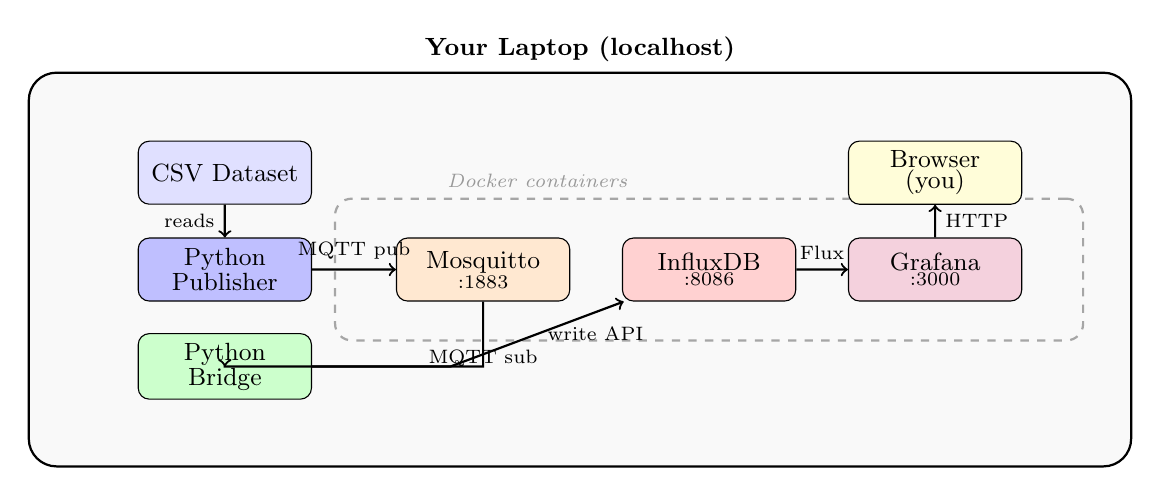
\begin{tikzpicture}[
        scale=0.82,
        every node/.style={font=\small},
        box/.style={draw, minimum width=2.2cm, minimum height=0.8cm, rounded corners},
        docker/.style={draw, dashed, thick, gray!70, rounded corners=6pt, inner sep=8pt},
    ]
        % --- Your laptop boundary ---
        \node[draw, thick, rounded corners=10pt, minimum width=14cm, minimum height=5cm,
              fill=gray!5, label={[font=\small\bfseries]above:Your Laptop (localhost)}] at (6,-1.5) {};

        % --- Docker boundary ---
        \node[docker, minimum width=9.5cm, minimum height=1.8cm,
              label={[font=\scriptsize\itshape, gray!80]above left:Docker containers}] at (8,-1.5) {};

        % --- Python scripts (outside Docker) ---
        \node[box, fill=blue!12]  (csv)    at (0.5, 0)    {CSV Dataset};
        \node[box, fill=blue!25]  (pub)    at (0.5,-1.5)  {\shortstack{Python\\[-2pt]Publisher}};
        \node[box, fill=green!20] (bridge) at (0.5,-3)    {\shortstack{Python\\[-2pt]Bridge}};

        % --- Docker services ---
        \node[box, fill=orange!18] (mqtt)    at (4.5,-1.5) {\shortstack{Mosquitto\\[-2pt]\scriptsize :1883}};
        \node[box, fill=red!18]    (influx)  at (8,-1.5)   {\shortstack{InfluxDB\\[-2pt]\scriptsize :8086}};
        \node[box, fill=purple!18] (grafana) at (11.5,-1.5) {\shortstack{Grafana\\[-2pt]\scriptsize :3000}};

        % --- Browser ---
        \node[box, fill=yellow!15] (browser) at (11.5, 0)  {\shortstack{Browser\\[-2pt](you)}};

        % --- Arrows ---
        \draw[->, thick] (csv) -- node[left, font=\scriptsize]{reads} (pub);
        \draw[->, thick] (pub) -- node[above, font=\scriptsize]{MQTT pub} (mqtt);
        \draw[->, thick] (mqtt) -- node[below, font=\scriptsize, yshift=-2pt]{MQTT sub} ++(0,-1.5) -| (bridge);
        \draw[->, thick] (bridge) -- ++(3.5,0) -- node[right, font=\scriptsize]{write API} (influx);
        \draw[->, thick] (influx) -- node[above, font=\scriptsize]{Flux} (grafana);
        \draw[->, thick] (grafana) -- node[right, font=\scriptsize]{HTTP} (browser);

    \end{tikzpicture}
    \end{center}

    \vspace{0.1cm}
    \begin{columns}
        \column{0.48\textwidth}
        \textbf{You write (Python):}
        \begin{itemize}
            \item \texttt{mqtt\_publisher.py} --- CSV $\rightarrow$ MQTT
            \item \texttt{mqtt\_bridge.py} --- MQTT $\rightarrow$ InfluxDB
        \end{itemize}

        \column{0.48\textwidth}
        \textbf{Docker runs for you:}
        \begin{itemize}
            \item Mosquitto broker (\texttt{:1883})
            \item InfluxDB time-series DB (\texttt{:8086})
            \item Grafana dashboards (\texttt{:3000})
        \end{itemize}
    \end{columns}
\end{frame}

\begin{frame}{Thursday Seminar: What You Will Accomplish}
    \begin{columns}
        \column{0.55\textwidth}
        \textbf{By end of the 1-hour session:}
        \begin{enumerate}
            \item Working MQTT pub/sub pipeline
            \item Real IoT data flowing into InfluxDB
            \item One live Grafana dashboard panel with an alert
        \end{enumerate}

        \vspace{0.3cm}
        \begin{alertblock}{Directly applicable to your project}
            In Weeks 12--14 you will replace the CSV with your real sensor.\\
            The rest of the pipeline stays \textbf{exactly the same}.
        \end{alertblock}

        \column{0.42\textwidth}
        \textbf{Seminar $\rightarrow$ Final Project:}

        \vspace{0.2cm}
        \begin{center}
        \footnotesize
        \begin{tabular}{ll}
            \toprule
            \textbf{Seminar} & \textbf{Your Project} \\
            \midrule
            CSV file & Real sensor \\
            Python script & MCU / SBC \\
            localhost & localhost or cloud \\
            1 room & your scenario \\
            \bottomrule
        \end{tabular}
        \end{center}

        \vspace{0.2cm}
        \textit{Same MQTT topics, same InfluxDB, same Grafana --- just a different data source.}
    \end{columns}
\end{frame}

%==============================================================================
\section{Week 12--13: MVP Build + Studio}
%==============================================================================

\begin{frame}{Weeks 12--13: Build Your MVP}
    \begin{center}
    \scriptsize
    \begin{tabular}{llll}
        \toprule
        \textbf{Week} & \textbf{Date} & \textbf{Session} & \textbf{What Happens} \\
        \midrule
        \multirow{3}{*}{\textbf{12}} & Mon 03/23 & Studio: Project Work & Hardware assembly, sensor bring-up \\
        & Tue 03/25 & Studio: Project Work & Sensor validation (datasheet vs.\ real) \\
        & Wed 03/26 & Studio: Project Work & MCU programmed to publish via MQTT \\
        \midrule
        \multirow{3}{*}{\textbf{13}} & Mon 03/30 & Studio: Project Work & MQTT $\rightarrow$ InfluxDB pipeline \\
        & Tue 04/01 & Studio: Project Work & Grafana dashboard + data quality \\
        & Wed 04/02 & Studio: Project Work & End-to-end integration + edge cases \\
        \bottomrule
    \end{tabular}
    \normalsize
    \end{center}

    \vspace{0.2cm}
    \begin{columns}
        \column{0.5\textwidth}
        \textbf{Week 12 (hardware + sensor):}
        \begin{itemize}
            \item Hardware assembled and tested
            \item Sensor reads correct values
            \item MCU/SBC programmed to publish via MQTT
            \item Broker running (local or cloud)
        \end{itemize}

        \column{0.5\textwidth}
        \textbf{Week 13 (pipeline):}
        \begin{itemize}
            \item Subscriber writing to InfluxDB
            \item Grafana showing live data
            \item Handle disconnects, bad readings
            \item Basic data quality: outlier, stuck sensor
        \end{itemize}
    \end{columns}

    \vspace{0.2cm}
    \begin{alertblock}{No demo deadline yet --- focus on building}
        I will be available during all studio sessions for hardware debugging, wiring help, protocol troubleshooting, and code review.
    \end{alertblock}
\end{frame}

\begin{frame}{Common Failure Modes (Plan Ahead)}
    \begin{columns}
        \column{0.5\textwidth}
        \textbf{Hardware:}
        \begin{itemize}
            \item Wrong voltage levels (3.3V vs 5V)
            \item Bad wiring (I2C pull-ups missing)
            \item Sensor not responding (wrong address)
        \end{itemize}

        \vspace{0.2cm}
        \textbf{Software:}
        \begin{itemize}
            \item WiFi config issues (eduroam!)
            \item MQTT topic typos (silent failure)
            \item Timestamp format mismatches
            \item InfluxDB bucket/token confusion
        \end{itemize}

        \column{0.5\textwidth}
        \textbf{How to debug:}
        \begin{itemize}
            \item \textbf{MQTT Explorer}: see all messages in real time
            \item \textbf{Serial monitor}: verify sensor readings before MQTT
            \item \textbf{InfluxDB Data Explorer}: check if data is arriving
            \item \textbf{Grafana}: if no data, the problem is upstream
        \end{itemize}

        \vspace{0.2cm}
        \begin{exampleblock}{Debug strategy}
            Always test each stage independently before connecting them. Sensor $\rightarrow$ Serial $\rightarrow$ MQTT $\rightarrow$ DB $\rightarrow$ Dashboard.
        \end{exampleblock}
    \end{columns}
\end{frame}

%==============================================================================
\section{Week 14: MVP Working Demo}
%==============================================================================

\begin{frame}{Week 14: MVP Working Demo}
    \begin{center}
    \footnotesize
    \begin{tabular}{llll}
        \toprule
        \textbf{Date} & \textbf{Session} & \textbf{What Happens} & \textbf{Deliverable} \\
        \midrule
        Mon 04/06 & Studio: Final Integration & Last fixes before demo & --- \\
        Tue 04/08 & Studio: Final Integration & Polish pipeline + dashboard & --- \\
        \textbf{Wed 04/09} & \textbf{MVP Working Demo} & \textbf{Show working sensor-to-dashboard} & \textbf{Live demo} \\
        \bottomrule
    \end{tabular}
    \normalsize
    \end{center}

    \vspace{0.2cm}
    \begin{center}
    \fcolorbox{milestoneborder}{milestonebg}{
    \begin{minipage}{0.85\textwidth}
        \vspace{0.2cm}
        \centering
        \large\textbf{Milestone: MVP Working Demo (Wed 04/09)}

        \vspace{0.2cm}
        \normalsize
        Show me (live, at your bench):
        \begin{enumerate}
            \item Sensor reading real data (not simulated)
            \item Data published over MQTT to a broker
            \item Data stored in InfluxDB (or your chosen DB)
            \item At least one Grafana panel showing live data
        \end{enumerate}

        \vspace{0.1cm}
        \textit{This is a checkpoint, not a grade. But if your pipeline is not working here, you are at risk for the final.}
        \vspace{0.2cm}
    \end{minipage}
    }
    \end{center}
\end{frame}

%==============================================================================
\section{Week 15: Pre-Demo Review + Report + Submissions}
%==============================================================================

\begin{frame}{Week 15: Pre-Demo Review + Report + Submissions}
    \begin{center}
    \footnotesize
    \begin{tabular}{llll}
        \toprule
        \textbf{Date} & \textbf{Session} & \textbf{What Happens} & \textbf{Deliverable} \\
        \midrule
        \textbf{Mon 04/13} & Pre-Demo Reviews & 10-min per team: show pipeline, get feedback & Slide deck draft \\
        \textbf{Tue 04/15} & \textbf{Final Submissions} & \textbf{All deliverables due by 11:59 PM} & \textbf{See next slide} \\
        Wed 04/16 & Final Clinic & Last-minute questions, demo prep & --- \\
        \bottomrule
    \end{tabular}
    \normalsize
    \end{center}

    \vspace{0.2cm}
    \textbf{Pre-Demo Review (Monday 04/13):}
    \begin{columns}
        \column{0.5\textwidth}
        \begin{enumerate}
            \item \textbf{5 min:} Live demo of your pipeline
            \begin{itemize}
                \item Sensor reading $\rightarrow$ MQTT $\rightarrow$ DB $\rightarrow$ Dashboard
                \item Explain each stage
            \end{itemize}
            \item \textbf{3 min:} Architecture diagram walkthrough
            \item \textbf{2 min:} Feedback from me + peers
        \end{enumerate}

        \column{0.5\textwidth}
        \textbf{I will evaluate:}
        \begin{itemize}
            \item Does the pipeline work end-to-end?
            \item Can you explain every design choice?
            \item What are the limitations you identified?
            \item What would you change with more time?
        \end{itemize}

        \vspace{0.1cm}
        \begin{exampleblock}{This is a dry run}
            Same format as your final demo, but with immediate feedback to improve.
        \end{exampleblock}
    \end{columns}
\end{frame}

\begin{frame}{Week 15: Final Submissions}
    \begin{center}
    \footnotesize
    \normalsize
    \end{center}

    \vspace{0.2cm}
    \begin{center}
    \fcolorbox{delivborder}{delivbg}{
    \begin{minipage}{0.85\textwidth}
        \vspace{0.2cm}
        \centering
        \large\textbf{Final Submission Deadline: Tuesday April 15, 11:59 PM}

        \vspace{0.2cm}
        \normalsize
        Submit to Canvas:
        \begin{enumerate}
            \item \textbf{Final Report} (PDF, LaTeX strongly recommended)
            \item \textbf{Source Code} (GitHub repo link or zip)
            \item \textbf{Demo Slide Deck} (for Week 16 presentation)
            \item \textbf{Architecture Diagram} (included in report and slides)
            \item \textbf{2-min Video} of your system working (backup if live demo fails)
        \end{enumerate}
        \vspace{0.2cm}
    \end{minipage}
    }
    \end{center}
\end{frame}

\begin{frame}{Final Report Structure}
    \textbf{Your final report must follow the PES structure, extended with implementation and results:}

    \vspace{0.2cm}
    \begin{columns}
        \column{0.5\textwidth}
        \begin{enumerate}
            \item \textbf{Problem Statement} (from PES)
            \begin{itemize}
                \item What you set out to solve
                \item Baseline, requirements, constraints
            \end{itemize}
            \item \textbf{System Architecture}
            \begin{itemize}
                \item Full pipeline diagram
                \item Justify every component choice
            \end{itemize}
            \item \textbf{Hardware Design}
            \begin{itemize}
                \item Sensor, MCU, comm module
                \item BOM with actual costs
                \item Wiring diagram or PCB layout
            \end{itemize}
            \item \textbf{Software Design}
            \begin{itemize}
                \item MQTT topic hierarchy
                \item Data format (JSON schema)
                \item Storage strategy (hot/cold)
                \item Dashboard design
            \end{itemize}
        \end{enumerate}

        \column{0.5\textwidth}
        \begin{enumerate}
            \setcounter{enumi}{4}
            \item \textbf{Results and Testing}
            \begin{itemize}
                \item Sensor accuracy (measured vs datasheet)
                \item Pipeline latency (end-to-end)
                \item Data quality report
                \item Dashboard screenshots
            \end{itemize}
            \item \textbf{Discussion}
            \begin{itemize}
                \item What worked, what didn't
                \item Limitations and failure modes
                \item What you would change
            \end{itemize}
            \item \textbf{AI Audit}
            \begin{itemize}
                \item What AI tools you used
                \item What they got wrong
                \item How you verified
            \end{itemize}
        \end{enumerate}

        \vspace{0.1cm}
        \begin{alertblock}{Grading emphasis}
            \textbf{Justification} and \textbf{test results} weigh more than feature count. A simple pipeline with excellent documentation beats a complex one with no testing.
        \end{alertblock}
    \end{columns}
\end{frame}

%==============================================================================
\section{Week 16: Final Presentations and Demos}
%==============================================================================

\begin{frame}{Week 16: Final Presentations and Demos}
    \begin{center}
    \footnotesize
    \begin{tabular}{llll}
        \toprule
        \textbf{Date} & \textbf{Session} & \textbf{What Happens} \\
        \midrule
        Mon 04/20 & FESTIVE (no class) & --- \\
        \textbf{Tue 04/22} & \textbf{Final Presentations I} & Teams 1--N/2 present + live demo \\
        \textbf{Wed 04/23} & \textbf{Final Presentations II + Retrospective} & Teams N/2+1--N + course retrospective \\
        \bottomrule
    \end{tabular}
    \normalsize
    \end{center}

    \vspace{0.2cm}
    \textbf{Presentation format (15 min per team):}
    \begin{columns}
        \column{0.5\textwidth}
        \begin{enumerate}
            \item \textbf{Pitch (3 min):} Problem, why it matters, your solution
            \item \textbf{Architecture (3 min):} Full pipeline walkthrough
            \item \textbf{Live Demo (5 min):} Show sensor $\rightarrow$ MQTT $\rightarrow$ DB $\rightarrow$ Dashboard working
            \item \textbf{Results + Lessons (2 min):} What worked, what didn't, key numbers
            \item \textbf{Q\&A (2 min):} Questions from me and peers
        \end{enumerate}

        \column{0.5\textwidth}
        \textbf{Grading criteria:}
        \begin{itemize}
            \item \textbf{30\%} --- Working end-to-end demo
            \item \textbf{25\%} --- Engineering rigor (justified choices, tested claims)
            \item \textbf{20\%} --- Presentation quality (clear, professional)
            \item \textbf{15\%} --- Data pipeline completeness (MQTT + storage + viz)
            \item \textbf{10\%} --- Handling of Q\&A
        \end{itemize}

        \vspace{0.1cm}
        \begin{alertblock}{Backup video}
            If your live demo fails, the 2-min video you submitted is your safety net. Without either: \textbf{0\%} on demo component.
        \end{alertblock}
    \end{columns}
\end{frame}

%==============================================================================
\section{Full Timeline Summary}
%==============================================================================

\begin{frame}{Full Timeline: Weeks 10--16 at a Glance}
    \vspace{0.1cm}
    \begin{center}
    \scriptsize
    \begin{tabular}{clp{5.5cm}p{4cm}}
        \toprule
        \textbf{Wk} & \textbf{Dates} & \textbf{Activities} & \textbf{Key Deliverable} \\
        \midrule
        \textbf{10} & 03/09--03/12 & Data Analytics wrap-up, Roadmap presentation & --- \\
        \midrule
        \textbf{11} & 03/16--03/20 & AI/MLOps lecture, MVP Spec (Wed), Cloud IoT Seminar (Thu) & \textbf{MVP Hardware Spec (Wed)} \\
        \midrule
        \textbf{12} & 03/23--03/26 & Studio: hardware build, sensor bring-up, MQTT & Sensors reading + publishing \\
        \midrule
        \textbf{13} & 03/30--04/02 & Studio: pipeline integration, data quality & --- \\
        \midrule
        \textbf{14} & 04/06--04/09 & Final integration + \textbf{MVP Working Demo (Wed)} & \textbf{MVP Working Demo (Wed)} \\
        \midrule
        \textbf{15} & 04/13--04/16 & Pre-demo review (Mon), submissions (Tue), clinic & \textbf{Final Report + Code + Video (Tue)} \\
        \midrule
        \textbf{16} & 04/20--04/23 & Final Presentations \& Demos (Tue--Wed) & \textbf{Live Demo + Pitch} \\
        \bottomrule
    \end{tabular}
    \normalsize
    \end{center}

    \vspace{0.2cm}
    \begin{alertblock}{Four key deadlines}
        \begin{enumerate}
            \item \textbf{Wed 03/19:} MVP Hardware Spec (so I can order parts over the weekend)
            \item \textbf{Wed 04/09:} MVP Working Demo (checkpoint --- show sensor-to-dashboard)
            \item \textbf{Tue 04/15:} Final Report + Code + Video (11:59 PM)
            \item \textbf{Tue/Wed 04/22--23:} Final Presentations (in person, no exceptions)
        \end{enumerate}
    \end{alertblock}
\end{frame}

\begin{frame}{What Your Demo Must Show}
    \textbf{Minimum viable demo (all teams):}

    \vspace{0.2cm}
    \begin{center}
    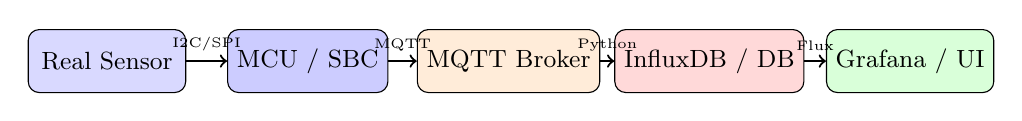
\begin{tikzpicture}[scale=0.85, every node/.style={font=\small}]
        \node[draw, fill=blue!15, minimum width=2cm, minimum height=0.8cm, rounded corners] (sens) at (0,0) {Real Sensor};
        \node[draw, fill=blue!20, minimum width=2cm, minimum height=0.8cm, rounded corners] (mcu) at (3,0) {MCU / SBC};
        \node[draw, fill=orange!15, minimum width=2cm, minimum height=0.8cm, rounded corners] (mqtt) at (6,0) {MQTT Broker};
        \node[draw, fill=red!15, minimum width=2cm, minimum height=0.8cm, rounded corners] (db) at (9,0) {InfluxDB / DB};
        \node[draw, fill=green!15, minimum width=2cm, minimum height=0.8cm, rounded corners] (dash) at (12,0) {Grafana / UI};

        \draw[->, thick] (sens) -- node[above]{\tiny I2C/SPI} (mcu);
        \draw[->, thick] (mcu) -- node[above]{\tiny MQTT} (mqtt);
        \draw[->, thick] (mqtt) -- node[above]{\tiny Python} (db);
        \draw[->, thick] (db) -- node[above]{\tiny Flux} (dash);
    \end{tikzpicture}
    \end{center}

    \vspace{0.2cm}
    \begin{columns}
        \column{0.5\textwidth}
        \textbf{Minimum (passing):}
        \begin{itemize}
            \item 1 real sensor reading real data
            \item Published via MQTT (any broker)
            \item Stored in a time-series DB
            \item 1 dashboard panel showing live data
            \item Can explain every design choice
        \end{itemize}

        \column{0.5\textwidth}
        \textbf{Excellent (A-grade additions):}
        \begin{itemize}
            \item Multiple sensors or multi-modal
            \item Data quality checks (outlier, stuck)
            \item Hot + cold path (InfluxDB + Parquet)
            \item Alerting rules in Grafana
            \item Professional dashboard with multiple panels
            \item Architecture doc with tradeoff analysis
        \end{itemize}
    \end{columns}
\end{frame}

\begin{frame}{Questions?}
    \begin{center}
        \Huge Questions?

        \vspace{0.8cm}
        \normalsize
        \textbf{Eduardo Baena}\\
        \texttt{e.baena@northeastern.edu}

        \vspace{0.5cm}
        \textit{EECE5155: Wireless Sensor Networks and the Internet of Things}\\
        Spring 2026

        \vspace{0.5cm}
        \textbf{Next hard deadline: MVP Hardware Spec --- Wednesday March 19}
    \end{center}
\end{frame}

\end{document}
